\documentclass{article}
\usepackage[utf8]{inputenc}
\usepackage{natbib}
\usepackage{graphicx}
\usepackage[export]{adjustbox}
\usepackage{graphicx,calc}
\newlength\myheight
\newlength\mydepth
\settototalheight\myheight{Xygp}
\settodepth\mydepth{Xygp}
\setlength\fboxsep{0pt}
\newcommand*\inlinegraphics[1]{%
  \settototalheight\myheight{Xygp}%
  \settodepth\mydepth{Xygp}%
  \raisebox{-\mydepth}{\includegraphics[height=\myheight]{#1}}%
}
\usepackage{wrapfig}
\usepackage{indentfirst}
\newcounter{question}
\setcounter{question}{0}
\usepackage{caption}
\usepackage{sidecap} 
\usepackage{float}
\usepackage[table]{xcolor}
\usepackage{longtable}
\usepackage{dblfloatfix} 
\usepackage{multicol}
\usepackage{hyperref}
\hypersetup{
    colorlinks=true,
    linkcolor=black,
    filecolor=magenta,      
    urlcolor=red,
}
\usepackage{tabularx}
\usepackage{booktabs} 
\usepackage{ltablex}
\usepackage{subfigure}
\usepackage{tikzpagenodes}
\renewcommand{\contentsname}{ Contents (Click to be redirected to specified page)}





\begin{document}
\date{February 2021}
\begin{center}

\section{Surviving The Fight Caves \& Jad}
Amy Nguyen
\\February 17, 2021
\end{center}
\begin{figure}[h!]
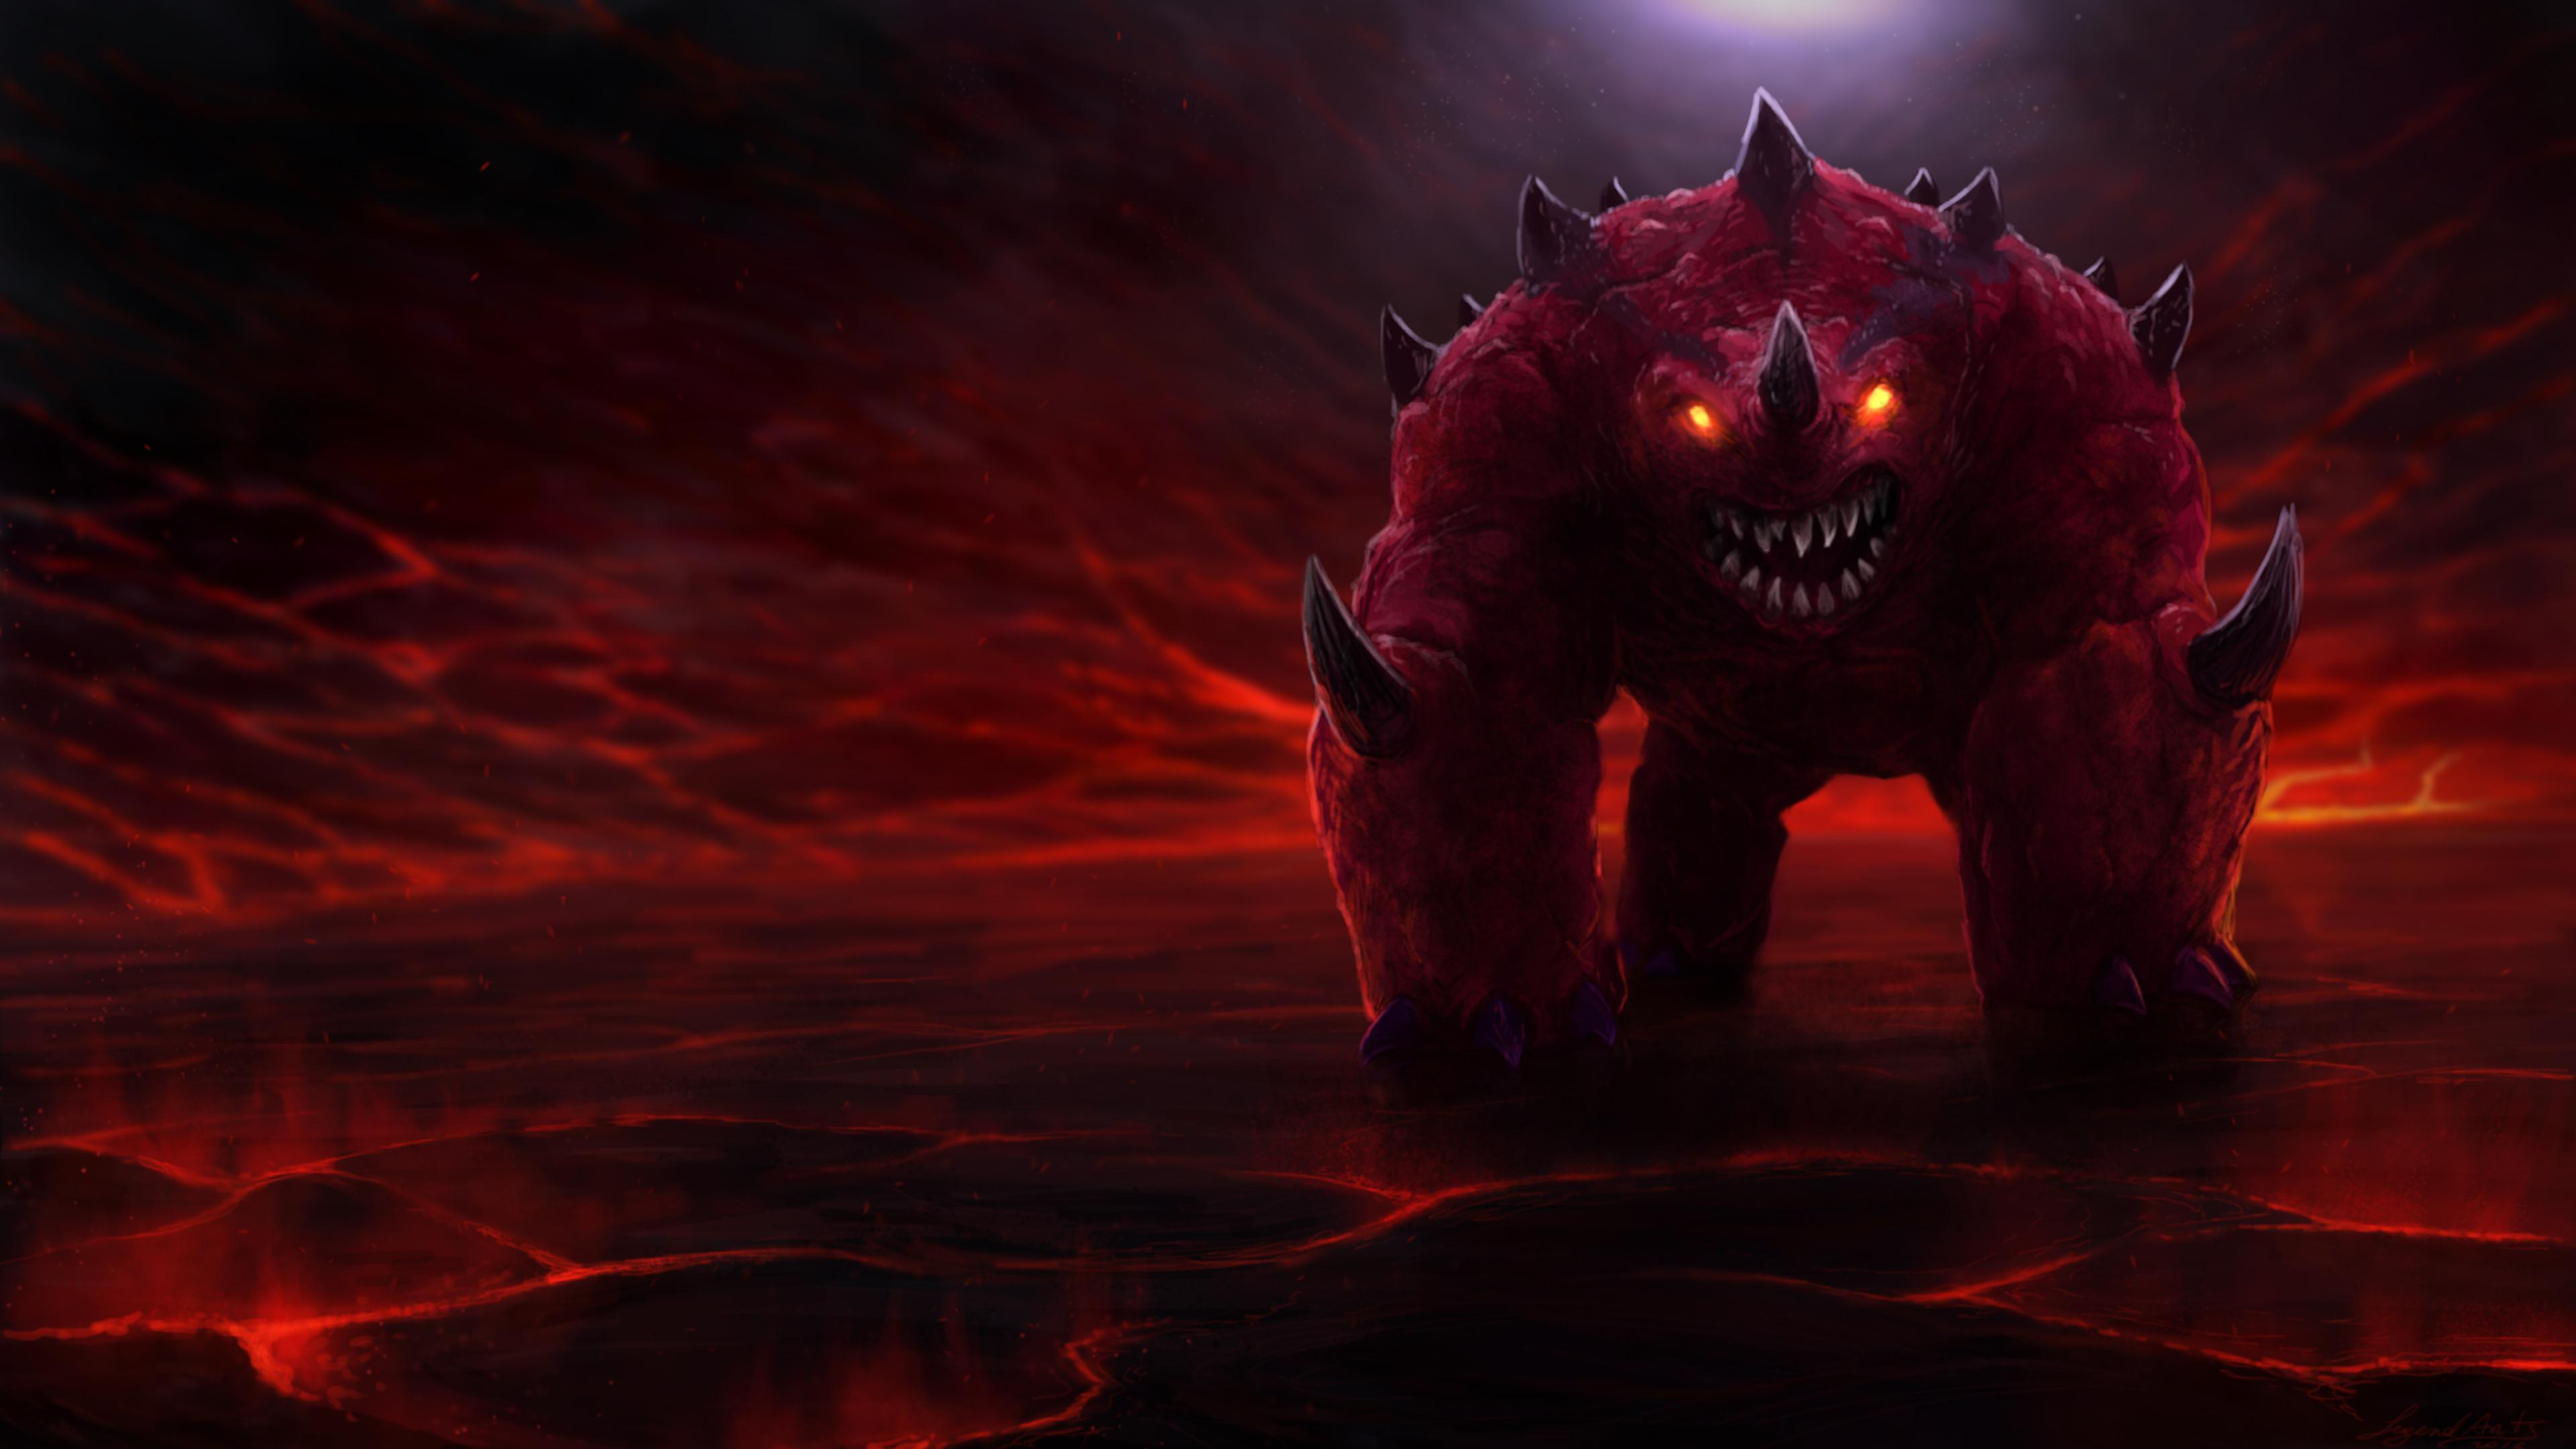
\includegraphics[width=130mm, scale=1.5]{jadtitle.jpg}
\end{figure}


\newpage
\tableofcontents
\newpage

\newcommand\Que[1]{%
   \leavevmode\par
   \stepcounter{question}
   \noindent
   \thequestion. Q --- \textbf{#1}\par}

\newcommand\Ans[2][]{%
    \leavevmode\par\noindent
   {\leftskip37pt
    A --- \textbf{#1}#2\par}}
    
\begin{figure}[h!]
\begin{center}

\includegraphics[scale=.7]{OSRS.png}
\end{center}
\end{figure}
\section{New to Old-School RuneScape?}
If you're reading this section, you must not be familiar with Old-School RuneScape at all! Don't worry, this will get you on your feet about the basics of RuneScape and maybe by the end you'll quest around Gielinor, (the world RuneScape takes place in) too!

\Que{What is Old-School RuneScape?}
\Ans{Old-School RuneScape is a Massive Online Multiplayer Role-Playing Game (MMORPG). 3 brothers, Andrew, Paul, and Ian Gower, created the foundations of RuneScape in their very own basement. Users can customize their own character, interact with other players, and do various of things such as embarking on quests around Gielinor. There are a few versions of RuneScape--the style being the main differentiating factor between them. Old-School RuneScape (OSRS) is one of the two playable versions-the other being RS3, RuneScape. OSRS is favored by its die-hard fans for love of its old-school graphic's aesthetics. It's a game that brings out old-school gaming nostalgia for all of its players!}

\Que{What is Gielinor?}
\begin{figure}[h!]
\begin{center}
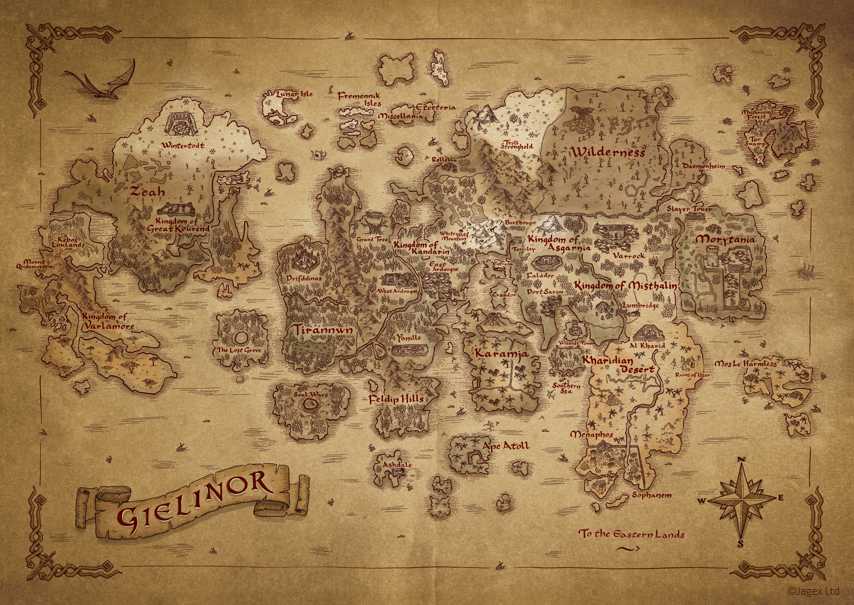
\includegraphics[scale=.27]{gil.png}
\end{center}
\end{figure}
\Ans{Gielinor is the world that RuneScape takes place in. It consists of 4 kingdoms(Misthalin, Asgarnia, Kandarin, \& Morytania), the Kharidian Desert, the tropical island Karamja, the Wilderness, ogre-inhabited Feldip Hills, elevan island of Tirannwn, Fremennik Province, and the continent of Zeah. }

\Que{I Finished Tutorial Island...What Now?}
\Ans{Funny enough, this is a reoccurring question that pops up from new players to old. The answer to that is: Anything you want! The OSRS is such an open-ended game that no one will have the same exact adventure as you! However, here are the main things you could be doing:
\begin{itemize}
    \item Working on Skilling 
    \begin{figure}[h!]
\begin{center}
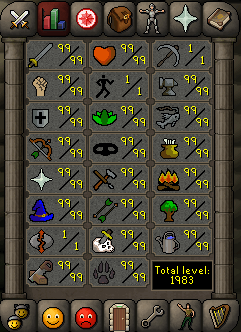
\includegraphics[scale=.5]{skills.png}
\end{center}
\end{figure}
    \begin{itemize}
        \item Working on stats that aren't related to your combat stats is called \emph{skilling}. These included skills such as farming, mining, thieving, herblore, construction, etc. However, some of these skills are only accessible to members--people that pay a monthly subscription to gain extra features in the game! It's only around 11 bucks so it doesn't hurt to support the game if you're player that wants the full RuneScape experience! \tiny jagex plz sponsor me
    \end{itemize}
    \item Working on Combat 
    \begin{itemize}
        \item Working on combat is one of the first things new players do. On World 301, the cow farms in Lumbridge are full of new players farming for their combat levels. Your combat insists of 7 skills.
        \begin{itemize}
            \item Attack, Strength, Defense, and Range are all types of fighting styles you can perform. Each style plays a different role in your stats. 
            \item Mage is another class of combat you can train on. All you need is a staff and runes to cast spells and you'll be on your way!
            \item Prayer isn't necessarily a combat staff but is there to aid you in combat with different buffs and debuffs granted as you level up. This can be achieved by burying bones. 
            \item Hitpoints refers to how much health points you have. As you level up your combat, your hitpoints also level up on their own speed. 
        \end{itemize}
    \end{itemize}
    \item Questing \inlinegraphics{quest}
    \begin{itemize}
        \item 
Questing is something you would either love or hate. Some of them can be very simple while others can be very tedious and long. You can check out the quests to do by opening up your quest book. At the end of each quest, you're awarded a number of quest points amongst other things for your time. Some quests have prerequisites so please be sure if you meet the stat requirements!
    \end{itemize}
\end{itemize}}
\begin{figure}[b!]
    \centering
    
\includegraphics{gno.png}
\end{figure}
\newpage 
\begin{center}
\section{Lore of Gielinor}
\noindent \tiny *Keep in mind how the creation of Gielinor came to be is argued amongst theorists and historians of RuneScape. The history of Gielinor can be biased and/or inaccurate due to it being passed down by tongue or is purely created by hypothesis. Walk the lands of Gielinor and learn about its tales to come to your own conclusions!
\end{center}

\vspace{2mm}
\subsection{The First Age - Creation}
\begin{wrapfigure}{R}{0.2\textwidth}
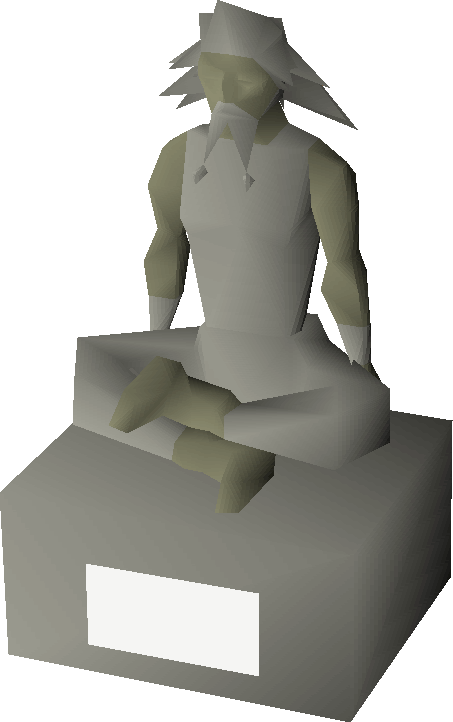
\includegraphics[width=0.2\textwidth,right]{guthix.png}
\caption*{\label{fig:guth}\small Statue of Guthix}
\end{wrapfigure}
\normalsize Gielinor is created by the 3 Gods--Saradomin--the God of Light, Zamorak--the God of Dark Fire(who became a god in the second age), and Guthix--the God of Balance. Throughout this period of time, the Gods took their time in creating the seas, lands, and populating the world we know as Gielinor with species Guthix deemed worthy. From what Gielinor theorists hypothesize, it took the Gods almost 4 thousand years to create Gielinor. At the end of the first age, Guthix was said to have went deep underground and began his long slumber until the end of The God Wars. 

\vspace{6mm}
\subsection{The Second Age - When the Gods Walked}
While Guthix is in his deep slumber, many other Gods arrived through the World Gate (allows access between worlds) and inhabited Gielinor, establishing their own territories and civilisations. This portal was closed off later on by Zaros, the God of Divine Darkness. Around this time he was gaining most of control of Gielinor until later he was overthrown by one of his generals Zamorak--who became a God from that outcome. During this time, the Gods and mortals interacted with one another a lot more freely and frequently. This is all to change in The Third Age.
\begin{figure}[h]
    \centering
    
\includegraphics[width=0.15\textwidth]{saradomin.png}
    \caption*{Statue of Saradomin}
    \label{fig:sara}
\end{figure}

\newpage
\begin{wrapfigure}{r}{.3\textwidth}

\includegraphics[width=0.45\textwidth]{zamorak.png}
\caption*{\label{fig:zam}Statue of Zamorak}
\end{wrapfigure} 
\section{The Third Age - The God Wars}
This approximately 4,000 year old period, The Third Age marked a time of great chaos for Gielinor. With Zaros' presence and control over Gielinor gone, other Gods fought over for complete control. Thus this resulted in The God Wars--a catastrophic battle between the Great Gods, so disastrous that moral beings like Humanity clung on for survival. Some living beings were far more unfortunate, perishing along with the havoc that ensued and even coming to extinctions. This war nearly destroyed Gielinor and woke Guthix up from his rest. Angered by the ruins that once made up a beautiful place he created, he used his power to cease the war completely. And from that he demanded that the Gods now only will have influence through their followers, having most of the Gods leaving Gielinor to back to their own home--the God Realm

\subsection{The Fourth Age - The Age of Mortals}
After the period of mass destruction was over, this 2,000 year old flourishing period for Gielinor's inhabitants took place. This healing period gave the mortal populace time to recuperate and build over destroyed civilizations. Due these races multiplying in size, they had to compete over the land's resources and territory. Humans, Gnomes, Goblins, Dwarves, Ogres and many other neighboring races fought against one another for these resources. They weren't just fight against other races but they also had civil battles as well. Due to the sheer amount of battles that took place, it hindered all of their progress to become more civilized. From this, individuals within their race split off into different tribes--fighting with neighboring ones for land and assets. This slow crawl of advancements in civilization was broken when a couple of human mages discovered how to make \textbf{runestones}\inlinegraphics{air.png}. This secret was kept amongst a group of mages, not letting this discovery fall into enemy hands as humans take their first steps in necromancy, beginning The Fifth Age-The Age of Humans.
\newpage

\begin{wrapfigure}{R}{.31\textwidth}
\centering
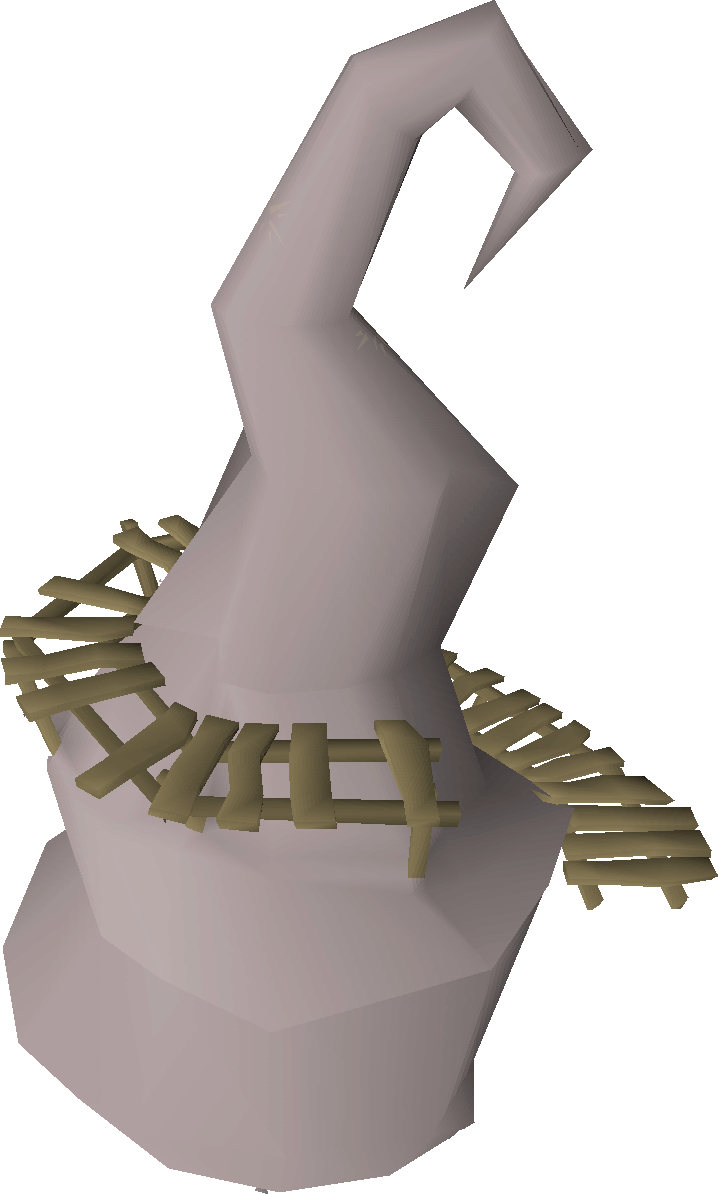
\includegraphics[width=0.2\textwidth]{runeessence.png}
\caption*{\small \label{fig:wise}Rune Essence}
\end{wrapfigure} 



\subsection{The Fifth Age - The Age of Humans}
\small \inlinegraphics{death.png}\inlinegraphics{fire.png}\inlinegraphics{air.png}This is the current age of Gielinor.\inlinegraphics{cosmic.png}\inlinegraphics{water.png}\inlinegraphics{nature.png}
\\ \normalsize The Age of Humans was dubbed as a secondary name since during this time the  major accomplishments that contributed to the dominance of the human population and power they gained over Gielinor. From here on, it'll count as the first years of humanity. In \textbf{Year 1}, this was when humans discovered rune essence (a mineral mined to convert  which lead to the discovery of magic. 
\begin{figure*}[h]
\begin{wrapfigure}{L}{.2\textwidth}
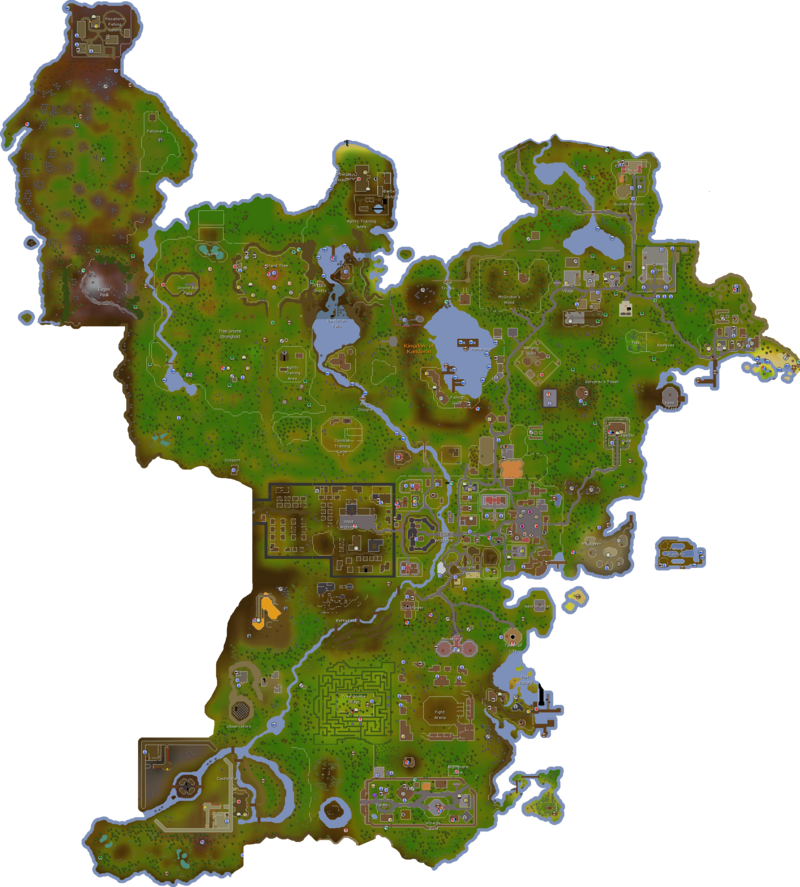
\includegraphics[width=.25\textwidth]{kar.png}
\caption*{\label{fig:kar}Kandarin}
\end{wrapfigure} 
\end{figure*}

In \textbf{Year 7}, the royal family of Carnillean decided to eridicate all evil in their area and named it Ardougne, which will be part of Kandarin, the largest nation in the world, later on in history. In \textbf{Year 19}, a very powerful demon named Delrith tried to destroy Varrock, the capital of the Kingdom of Misthalin. A brave warrior named Wally however managed to stop this demon. During \textbf{Years 42-62}, Barbarians felt that the act of runecrafting (creating runes for magic) should be left for the Gods. Thus havoc insued during their campaign for their beliefs, they parade across northern Kandarin and Asgarnia. However at \textbf{Year 62}, they were forced to retreat into their own civilization--the Barbarian Village. By \textbf{Year 60-70}, Imcando dwarves were nearly extinct from the Barbarian invasions. 

\begin{wrapfigure}{R}{.1\textwidth}

\includegraphics[width=.12\textwidth]{dai.png}
\caption*{\label{fig:dai}Daigon'hai Robe}
\end{wrapfigure}
At the \textbf{Year 70}, Daigon'hai, a group of Zamorak followers made a Saradomin statue in Varrock which hid the entrance to their secret hideout, the Tunnel of Chaos. During this year both Saradomin and Zamorak wizards worked together to study magic at the Tower of Life located on an island. This was until the power hungry Zamorak wizards burned down the Tower of Life, destroying countless of tomes. This sparked riots at Varrock which led to their discovery of the secret hideout and their plans to resurrect Zamorak's will. Both of these actions from the Zamorak people were unforgivable and people drove them out of Varrock and killing two of the four elders of Dagon'hai. During \textbf{Year 136}, the king that ruled Kandarin died and his sons couldn't decide who will be the successor so they ended up dividing Ardougne in half.
\begin{wrapfigure}{r}{.2\textwidth}
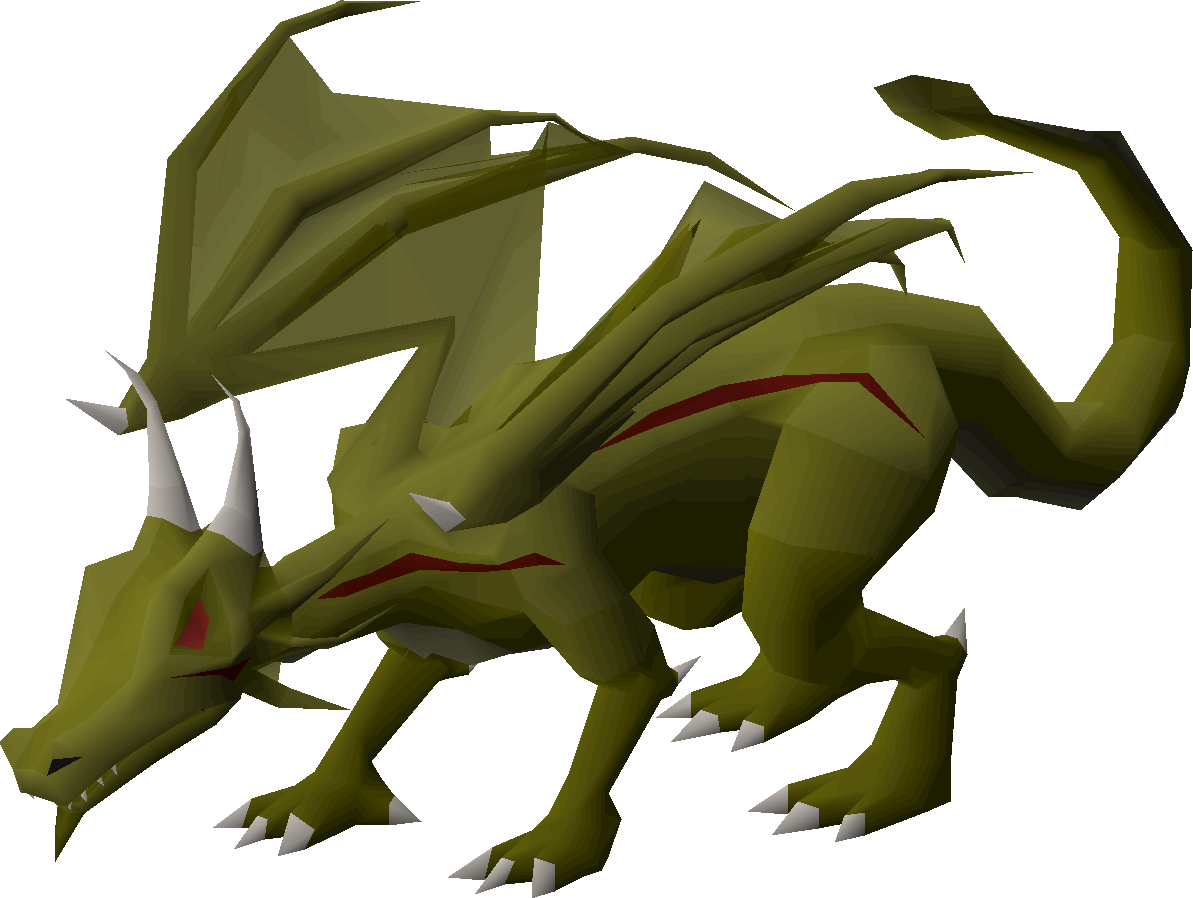
\includegraphics[width=.25\textwidth]{Elvarg.png}
\caption*{\label{fig:drag}Elvarg}
\end{wrapfigure} 
During \textbf{Year 139}, there was a thriving community that lived on an island with an active volcano named Crandor. The community was full of ancient wizards and adventurers. However, one adventurer decided to explore deep down in the volcano and accidently woken up a dragon named Elvarg up. She wrecked havoc upon Crandor and killed everyone but 3 wizards named Thalzar, Lozar, and Melzar. The three split up the last remaining map of Crandor and hid them individually--kepting the incident a secret. From \textbf{Year 150-159}, King Kharedst dies, leaving that the last ruler of their monarch. Now the Kingdom of Great Kourend is ruled by the Kourend City Council. Between these years, \textbf{Year 154} was when a necromancer, siding with Zamorak followers, plans an attack on Varrock who successfully defends their capital.A year after, \textbf{Year 155}, marks the end of the Nomads. They settle down after the abduction of their chieftain's daughter. \textbf{Year 169} marks the present day in Gielinor. 
\newpage
\section{Introduction to The Fight Caves}
\begin{wrapfigure}{L}{.28\textwidth}

\includegraphics[width=.22\textwidth]{tzhaar.png}
\caption*{\small \label{fig:dai}TzHaar-Ket}
\end{wrapfigure}
If you're reading this section of the document, you must be curious about the beloved fire cape. To achieve the fire cape, one must travel to Mor Ul Rek (located under the Karamaja volcano) also known as TzHaar City--populated by the TzHaar people. The TzHaar are peaceful  yet strong golems made out of magma and obsidian that have existed for thousands of years. Most of their history is a mystery however they have memories that last for thousands and thousands of years since they have the capability to transfer their memories from one another.
\begin{figure*}[h]
\begin{wrapfigure}{R}{.2\textwidth}

\includegraphics[width=.21\textwidth]{rock.png}
\caption*{\small \label{fig:dai}Dead TzHaar}
\end{wrapfigure}

Although their life expectancy is unknown, it is estimated that the TzHaar can live for thousands of years, When they die, their body hardens up and their mind is still intact with it. They're either left like statues or are converted into the holy TzHaar's ancient currency called Tokkul.\inlinegraphics{tokkul.png} They have a 4 part caste system from highest to lowest rank: TzHaar-Ket (The Guardians), TzHaar-Xil (The Hunters), TzHaar-Mej (The most wisest TzHaar and The Governing Class), and the TzHaar-Hur(The Craftmans). To gain access to the rest of Mor Ul Rek, you must prove your strength by defeating Jad and presenting them the fire cape. \\ 
\\Now the question is, \textit{are you worthy enough to wear the fire cape?}
\end{figure*}
\begin{figure}
    \centering
    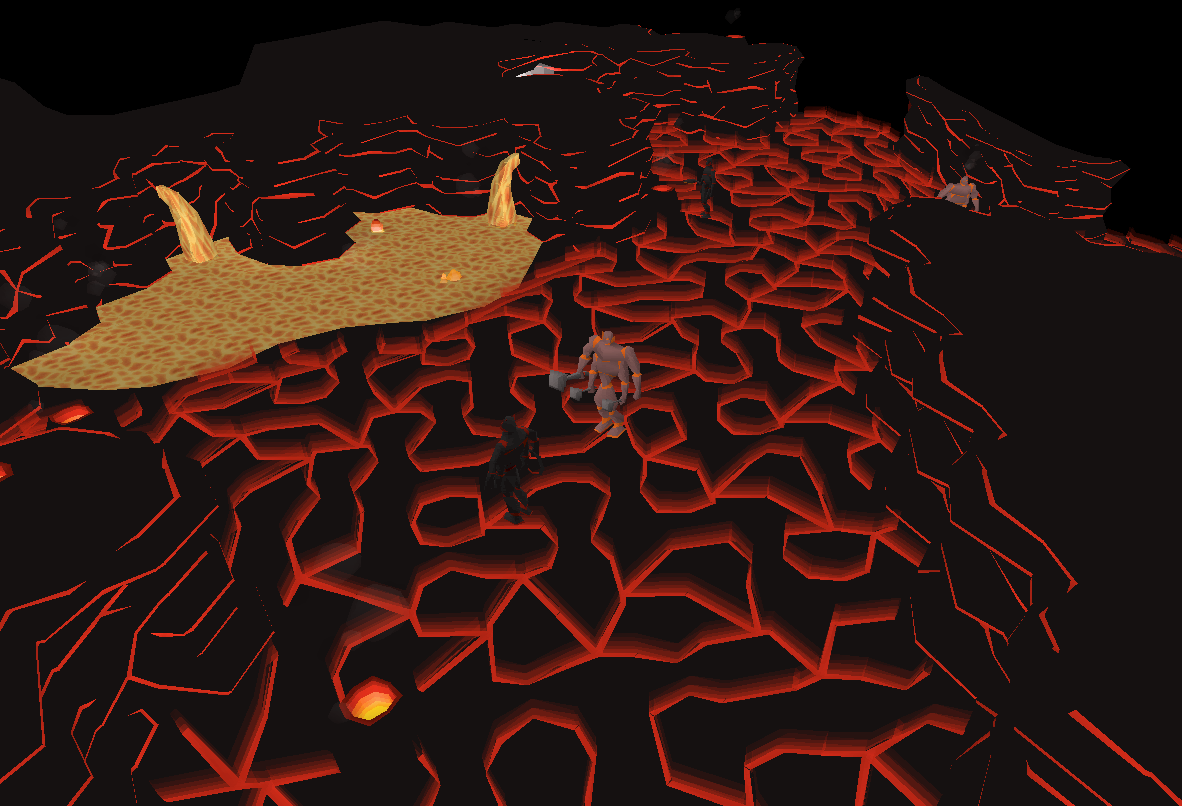
\includegraphics[scale=.16]{city.png}
    \caption*{Mol Ul Rek}
    \label{fig:my_label}
\end{figure}
\newpage
\begin{centering}
\section{Preparations}
\subsection{Stats Required to Survive} 
\end{centering}
\par If you wish to survive through The Fight Caves and defeat Jad, these are the minimum stats you need. \textbf{Please notice that this is not recommended!} Having the bare minimum stats and supplies will make the fight \textit{double} the average time and a lot more tedious compared to  the preferred stats and equipment.
\begin{center}
 \begin{tabular}{||c c ||} 
 \hline
Minimum  & Preferred  \\ [0.5ex] 
 \hline
\inlinegraphics{range.png} 61 Range & \inlinegraphics{range.png} 75 Range \\ 
 \hline
\inlinegraphics{defense.png} 40 Defense & \inlinegraphics{defense.png} 70+ Defense \\
 \hline
\inlinegraphics{prayer.png} 43 Prayer & \inlinegraphics{prayer.png} 53+ Prayer \\ [1ex]
 \hline
\end{tabular}
\end{center}
\subsection{Equipment Required}
To increase your success rate in The Fight Caves, you must have proper armor and weaponry according to your stats. Look below for different setups and choose what caters most to your needs. \textbf{Keep in mind that you need 75 range to wield the Toxic Blowpipe! The best armor has specific stat requirements to be met so make sure you check!} 
\begin{center}
\setlength{\arrayrulewidth}{1mm}
\setlength{\tabcolsep}{14pt}
\renewcommand{\arraystretch}{1}
{\rowcolors{3}{green!80!yellow!50}{green!70!yellow!40}
\begin{longtable}{ |p{1cm}|p{2cm}|p{2cm}|p{2cm}| }
\hline
\multicolumn{4}{|c|}{Most to Least Effective} \\
\hline
Slots & Best & Optimal & Most Affordable \\
\hline
Head & Armadyl Helmet & Blessed Coif/Archer Helm (ranged), Verac's Helm (tank) & Neitiznot \\
\hline
Body & Armadyl Chestplate & Blessed D'hide Body & Karil's leathertop/D'hide Body \\
\hline
Legs & Armadyl Chainskirt & Blessed Chaps & Verac's Plateskirt  \\
\hline
\endfirsthead
Arms & Barrows Gloves & Blessed Vambraces & Spikey Vambraces\\
\hline
Feet & Pegasian Boots & Blessed Boots & Devout Boots/Bandos Boots \\
\hline
Weapon & Toxic Blowpipe & Dragon Crossbow & Rune Crossbow \\

Shield & Twisted Buckler & Odium Ward & Toktz-ket-xil\\
\hline
Rings & Archers Ring & Ring of Suffering(i) & Any \\
\hline
Back & Ava's Assembler & Ava's Device & Ranging Cape \\
\hline
Necklace & Necklace of Anguish & Amulet of Fury & Amulet of Glory \\

Extras & Adamant darts \& Zul'Rah Scales & Diamond (e) Bolts & Broad Bolts \\
\hline
\end{longtable}
}
\end{center}
\vspace{2mm}
\subsection{Inventory}
\begin{wrapfigure}{L}{.28\textwidth}
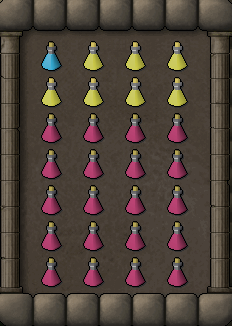
\includegraphics[width=.22\textwidth]{inv.png}
\caption*{\small \label{fig:dai}Example of Inventory}
\end{wrapfigure}
\normalsize \textit{Before entering The Fight Caves, eat 1 Angler fish and drink a sip of type of Ranging Potion to give yourself a head start in bonus HP and stats.}
To stay alive, you need a range of Saradomin Brews, Ranging Potions, and Super Restores. Buy 2 ranging potions or bastion potions for extra defense. Then have 12 Saradomin Brews and then fill up the rest of the inventory with Super Restores. If you find that you don't need more of one thing than the other, feel free to switch around your inventory. Keep notice of how much Super Restores (used to restore Prayer \& stats) and Saradomin Brews (used to restore HP) you use as you progress through the waves. It is recommended strongly that you have at least 3-4 brews and Super Restores when you get to Jad. \textbf{Always remember to drink a 3:1 sip ratio of Saradomin Brews:Super Restores since the Saradomin Brews debuffs your stats.}
\subsection{Getting there}
The most easiest way to get to The Fight Caves is to go under the minigames \inlinegraphics{minigame.png} and look for "TzHaar Fight Pit" and teleport there. Once there, run up the path and you will see a bank and the entrance to The Fight Cave. Keep in mind that there is a 20 minute cool down for when you can use the minigame teleport again! Another method to get there is buying the Amulet of Glory and teleporting to Karamja. Once you're there, run towards the volcano and climb down the hole with the rope you used in Dragon Slayer I.
\newpage
\section{Layout of The Fight Caves}
\begin{wrapfigure}{L}{.6\textwidth}
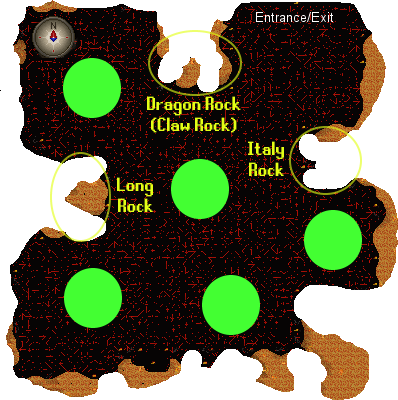
\includegraphics[width=.6\textwidth]{Fight_Caves_Map.png}
\end{wrapfigure}
Here is what The Fight Caves looks like on the map. There are a few things on the map that you should be familiar with so you can use it to your advantage. The Italy Rock can be used to trap melee monsters from getting into melee range and can also cut the enemy's field of view so they don't aggro you thus giving you time for a breather. Use the environment to your advantage to prepare for the next up coming wave or to take as little as damage as possible. Try not to take your first sip of brew or super restore until wave 30. The Italy Rock, Long Rock, and Dragon Rock can all be used to block the pathing melee monsters or to stop them from aggroing you.
There are 62 waves of monsters you must fight until you get to face Jad.
\\There'll be different combinations of them so you must know which monster to prioritize and kill first! Also remember you can log out at the end of every wave to save your progress or if you wish to take a break. Just click on the logout button only once and your progress will be saved. Note that you will be spawned into the following wave when you do log back in so be prepared! Here are the monsters you will be facing and what to do against them.
\newpage

\textbf{The killing order is \underline{29314} (numbers are based off of their level). }

\begin{multicols}{2}
  \null \vfill
  
\includegraphics[width=.3\textwidth]{tzkih.png}
  \vfill \null
\columnbreak
  \null \vfill
  \begin{itemize}
    \item \underline{Tz-Kih}
    \item Level 22, \textbf{KILL FIRST}
    \item Drains prayer by 1 every melee--\textbf{do NOT let it touch you.} Use range to kill--hit it then run away to maintain distance.
    \item Attack Style - Melee
    \item Max hit of 4
  \end{itemize}
  \vfill \null
\end{multicols}

\begin{multicols}{2}
  \null \vfill
  
\includegraphics[width=.3\textwidth]{tzkek.png}
  \vfill \null
\columnbreak
  \null \vfill
  \begin{itemize}
    \item \underline{Tz-Kek}
    \item Level 45, \textbf{KILL LAST}
    \item After \textit{killing it, it will break into 4 smaller level 22 Tz-Keks}
    \item Attack Style - Melee
    \item Recoil damage of 1
    \item Max hit of 7
  \end{itemize}
  \vfill \null
\end{multicols}

\begin{multicols}{2}
  \null \vfill
  
\includegraphics[width=.3\textwidth]{kek22.png}
  \vfill \null
\columnbreak
  \null \vfill
  \begin{itemize}
    \item \underline{Tz-Kek}
    \item Level 22, \textbf{KILL LAST}
    \item Spawns as a pair after killing level 45 Tz-Kek
    \item Attack Style - Melee
    \item Max hit of 4
    
  \end{itemize}
  \vfill \null
\end{multicols}

\textbf{The killing order is \underline{29314} (numbers are based off of their level). }
\begin{multicols}{2}
  \null \vfill
  
\includegraphics[width=.3\textwidth]{tokxil.png}
  \vfill \null
\columnbreak
  \null \vfill
  \begin{itemize}
    \item \underline{Tok-Xil}
    \item Level 90, \textbf{KILL SECOND}
    \item Pray range but after wave 30, pray magic and kill Tok-Xil first since it will do a good amount of damage to you
    \item Attack Style - Range, Melee
    \item Max hit of 13
  \end{itemize}
  \vfill \null
\end{multicols}

\begin{multicols}{2}
  \null \vfill
  
\includegraphics[width=.3\textwidth]{yt.png}
  \vfill \null
\columnbreak
  \null \vfill
  \begin{itemize}
    \item \underline{Yt-MejKot}
    \item Level 280, \textbf{KILL SECOND LAST}
    \item Use the environment/terrain to your advantage so you won't take damage from it \textit{ex. Italy Rock}
    \item Can heal itself and others around it
    \item Attack Style - Melee
    \item Max hit of 25
  \end{itemize}
  \vfill \null
\end{multicols}
\newpage

\begin{multicols}{2}
  \null \vfill
  
\includegraphics[width=.3\textwidth]{ketzek.png}
  \vfill \null
\columnbreak
  \null \vfill
  \begin{itemize}
    \item \underline{Ket-Zek}
    \item Level 160, \textbf{KILL THIRD}
    \item Spawns in at wave 30--does a TON of damage so be sure to pray magic and never take it off when it's alive!
    \item Make sure to stay outside of its melee range. Its bite will deal a ton of damage!
    \item Attack Style - Range, Melee
    \item Max hit of 54
  \end{itemize}
  \vfill \null
\end{multicols}
 \normalsize At wave 62 there will be 2 different colored Ket-Zeks that spawn in. Pay attention to where the orange Ket-Zek spawns since that will be where Jad spawns. If the orange Ket-Zek spawns near any terrain, use that to your advantage. You can hide behind the terrain wall to prepare for Jad after you kill the last Ket-Zek. When you're ready, turn your sound on if you haven't already and pray range. Jad can attack with either range or mage first but it's important to pray range first since you can only hear the attack when its too late. Whereas for mage, you can hear the attack before hand, giving you a second to switch prayers before it hits you. 

 \vspace{5mm}
 \centering
\href{https://oldschool.runescape.wiki/index.php?title=File\%3ATzTok-Jad_Ranged_attack.ogg}
    {Click here to listen to what Jad's range attack sounds like}

    \vspace{2mm}
\href{https://oldschool.runescape.wiki/index.php?title=File\%3ATzTok-Jad_Magic_attack.ogg}
    {Click here to listen to what Jad's mage attack sounds like}
    \begin{figure}[b!]
        \centering
        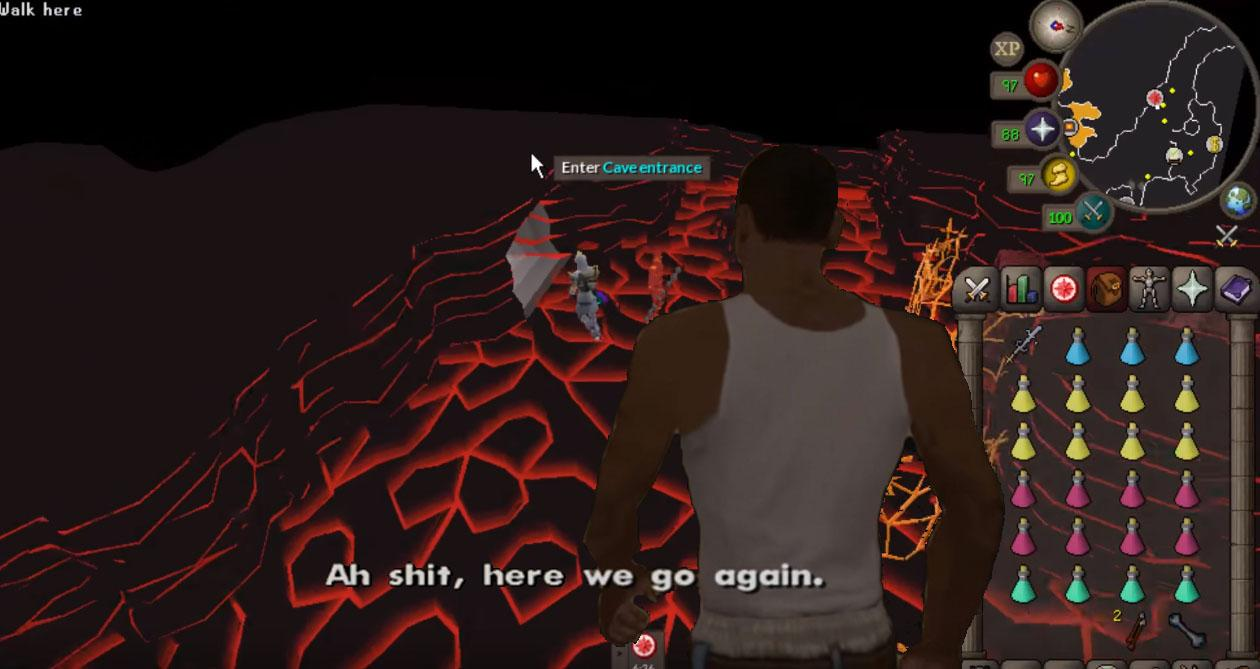
\includegraphics[scale = .2 ]{ahshit.jpg}
    \end{figure}
\newpage
\begin{center}
\section{Wave 63 - Jad fight}
\end{center}

\begin{multicols}{2}
  \null \vfill
  
\includegraphics[width=.3\textwidth]{jad.png}
  \vfill \null
\columnbreak
  \null \vfill
  \begin{itemize}
    \item \underline{TzTok-Jad}
    \item Level 702
    \item Spawns in where the orange Ket-Zek spawns at wave 62 
    \item Stay out of melee range. Jad switches from 2 attack styles--Range and Magic.
    \item Attack Style - Range, Magic, Melee
    \item Max hit of 54
  \end{itemize}
  \vfill \null
\end{multicols}


\begin{multicols}{2}
  \null \vfill
  
\includegraphics[width=.3\textwidth]{yt2.png}
  \vfill \null
\columnbreak
  \null \vfill
  \begin{itemize}
    \item \underline{Yt-HurKot}
    \item Level 108
    \item 4 of them spawns in when Jad is half HP. They will heal him to full if he is in range of them. If they're killed, they will respawn back. 
    \item Attack Style - Melee
    \item Max hit of 14
  \end{itemize}
  \vfill \null
\end{multicols}
\newpage

\section{Waves \& Monsters}
Here is a list of all the waves and monsters that spawn each wave. There will also be tips on how to handle each wave. The monsters will be referred as their level. If there is row that says N/A, assume nothing new is to be done. \textbf{Remember the 29314 rule!}
\begin{table}[!htbt]
    \begin{tabular}{  l  p{3.4cm}  p{3.4cm} }
        \toprule
\textbf{Wave}      
& \textbf{Monster}   
& \textbf{Information} \\\midrule
1 & 22 & Hit \& Run. Don't let it touch you. \\\hline

2 & 22, 22 & N/A  \\\hline

3 & 45 & N/A \\\hline

4 & 45, 22 & Kill 22 first then 45 \\\hline

5 & 45, 22, 22 & N/A \\\hline

6 & 45, 45 & After killing the last 45, pray \textbf{Protect from Missiles} \\\hline

7 & 90 & Use Protect from Missiles. You can prayer flick to conserve prayer.\\\hline

8 & 90, 22 & Kill 22 first, keep praying protect from missiles \\\hline

9 & 90, 22, 22 & N/A \\\hline

10 & 90, 45 & Kill 90 first before killing the 45 \\\hline

11 & 90, 45, 22 & Kill 22, 90, then 45 \\\hline

12 & 90, 45, 22, 22 & N/A \\\hline

13
& 90, 45, 45
& Kill 90 first then 45 \\\hline

14
& 90, 90
& N/A \\\hline

15 
& 180
& You can pray melee when the level 90 isn't present if you're afraid of getting melee'd by the 180. The best method to kill the 180 is to use the Italy Rock or any other terrain to trap it and ranging it without getting hit. \\
        \bottomrule
        \multicolumn{2}{r}{\footnotesize(Continued on next page...)}
    \end{tabular}
\end{table}
\newpage

\huge  \inlinegraphics{jad.png}  \textbf{Remember the \underline{29314} rule!}\inlinegraphics{jad.png}    

\begin{table}[!htbt]
    \begin{tabular}{  l  p{3.4cm}  p{3.4cm} }
        \toprule
\textbf{Wave}      
& \textbf{Monster}   
& \textbf{Information} \\\midrule
21
& 180, 45, 45
& N/A \\\hline

22 & 180, 90 & Pray range and kill the level 90 first. Use the 90 to block the 180 from meleeing you.  Remember to not get too close to the 90 to avoid being melee'd.\\\hline

23 & 180, 90, 22 & Pray range and kill the level 22 first. Then kill the 90 and then the 180. \\\hline

24 & 180, 90, 22, 22 & N/A \\\hline

25 & 180, 90, 45 & Pray range and kill the 90 first, then the 180 and lastly the 45. \\\hline

26 & 180, 90, 45, 22 & Pray range and kill the 22, 90, 180, then the 45. \\\hline

27& 180, 90, 45, 22, 22& N/A \\\hline

28 & 180, 90, 45, 45 & Pray range and kill the level 90, Then kill the 180 and then the two 45s. \\\hline

29 & 180, 90, 90 & Pray range and kill both the level 90s before you kill the 180. \\\hline

30 & 180, 180 & Take a sip of your Saradomin brew and Super Restore if needed. Remember the 3:1 Sara brew: Super Restore ratio! After killing the last 180, immediately pray mage. NEVER take your prayer off of mage if the level 360 is alive! \\\hline
        \bottomrule
        \multicolumn{2}{r}{\footnotesize(Continued on next page...)}
    \end{tabular}
\end{table}
\newpage


\huge  \inlinegraphics{jad.png}  \textbf{Remember the \underline{29314} rule!}\inlinegraphics{jad.png}    

\begin{table}[!htbt]
    \begin{tabular}{  l  p{3.4cm}  p{3.4cm} }
        \toprule
\textbf{Wave}      
& \textbf{Monster}   
& \textbf{Information} \\\midrule
31 & 360 & \textbf{Always keep protect mage on whenever 360 is alive.} Be sure to stay out of melee range because it will bite and do a ton of damage! \\\hline

32 & 360, 22 & Kill the 24 first. \\\hline

33 & 360, 22, 22 & N/A \\\hline

34 & 360, 45 & Kill the 360 and then the 45. \\\hline

35 & 360, 45, 22 & Kill the 22, 360, then 45. \\\hline

36 & 360, 45, 22 & N/A \\\hline

37 & 360, 45, 45 & Keep your HP in check! Heal before the next wave. \\\hline

38 & 360, 90 & Kill the 90 first before killing the 360. \\\hline

39 & 360, 90, 22 & Kill the 22, 90, then the 360. Don't let the 90 get close to you--it's melee hurts! \\\hline

40 & 360, 90, 22, 22 & N/A \\\hline

41 & 360, 90, 45 & Kill the 90, 360, then the 45. \\\hline

42 & 360, 90, 45, 22 & Kill the 22, 90, 260, then 45. \\\hline

43 & 360, 90, 45, 22, 22 & N/A \\\hline

44 & 360, 90, 45, 45 & N/A \\\hline

45 & 360, 90, 90 & Kill the 90s first. This can be done by either using the 360 to body block them from meleeing you or using the map in your favor. Don't let the 90s get close to you! \\\hline


      \bottomrule
        \multicolumn{2}{r}{\footnotesize(Continued on next page...)}
    \end{tabular}
\end{table}
\newpage


\huge  \inlinegraphics{jad.png}  \textbf{Remember the \underline{29314} rule!}\inlinegraphics{jad.png}    
\begin{table}[!htbt]
    \begin{tabular}{  l  p{3.4cm}  p{3.4cm} }
        \toprule
\textbf{Wave}      
& \textbf{Monster}   
& \textbf{Information} \\\midrule

46 & 360, 180 & Kill the 180 first since it's the only one doing damage to you. \\\hline

47 & 360, 180, 22 & Kill the 22, 180, then the 360. \\\hline

48 & 360, 180, 22, 22 & N/A \\\hline

49 & 360, 180, 45 & Kill the 180, 360, then 45. \\\hline

50 & 360, 180, 45, 22 & Kill the 22 first! \\\hline

51 & 360, 180, 45, 22, 22 & N/A \\\hline

52 & 360, 180, 45, 45 & N/A \\\hline

53 & 360, 180, 90 & Kill the 180 first. While doing so, try to trap the 90 behind it so it won't be in melee range. After that, trap the 90 again either with the 360 or using the rocks to kill it. \\\hline

54 & 360, 180, 90, 22 & N/A \\\hline

55 & 360, 180, 90, 22, 22 & N/A \\\hline

56 & 360, 180, 90, 45 & N/A \\\hline

57 & 360, 180, 90, 45, 22 & N/A \\\hline

58 & 360, 180, 90, 45, 22 & N/A \\\hline

59 & 360, 180, 90,  45, 45 & N/A \\\hline

60 & 360, 180, 90, 90 & Keep away from the level 90s. Try to trap them in between the 180. 360, or use the rocks to your advantage. \\\hline

61 & 360, 180, 180  & N/A \\\hline 
     \bottomrule
        \multicolumn{2}{r}{\footnotesize(Continued on next page...)}
    \end{tabular}
\end{table}
\newpage

\huge  \inlinegraphics{jad.png}  \textbf{Remember the \underline{29314} rule!}\inlinegraphics{jad.png}    
\begin{table}[!htbt]
    \begin{tabular}{  l  p{3.4cm}  p{3.4cm} }
        \toprule
\textbf{Wave}      
& \textbf{Monster}   
& \textbf{Information} \\\midrule
62 & 360, 360 & Keep in mind where the \textbf{orange} 360 spawns. That will be where Jad will spawn so plan and prepare accordingly when you get the last hit off of the orange one. If it spawns in a corner behind any rock formations, hide behind the other wall so Jad won't see you as he spawns in. This'll give you time to prepare for him. Pot up and get ready...! \\\hline

63 & 702 (Jad) 108 x4 (healers) & See next page for help on Jad.

    \end{tabular}
\end{table}

\begin{figure}[!h]
    \centering
    
\includegraphics[scale = .8]{lookout.png}
\end{figure}
\newpage


\section{Fighting TzTok-Jad} 
\begin{wrapfigure}{R}{.2\textwidth}

\includegraphics[width=.2\textwidth]{jad.png}
\end{wrapfigure}

\par \normalsize Obtaining the Fire Cape is one of the goals a dedicated RuneScape player would work towards. Defeating Jad separates the newer players to the experienced and opens up a new level of intensity PvM (player vs. monsters) has to offer. Because of that, many players take on the chance of getting the Fire Cape, adorning it on their character as they walk around in Gielinor for all to see. Not only that, but getting the Fire Cape is needed to get the Inferno Cape--Something that the very experienced players try to get! However, this guide will only tell you how to get the Fire Cape, not the Inferno. Here are some things you need to learn to have a higher success rate in beating Jad or reasons why you could be having trouble beating him. 
\subsection{Prayer Flickering}
\begin{wrapfigure}{L}{.399\textwidth}

\includegraphics[width=.1\textwidth]{protectmage.png}
\small \caption*{Protect From Magic}
\end{wrapfigure}
\par To survive Jad, you must know how to prayer flick. 
Prayer flicking is switching to different prayers or switching a prayer on and off in quick secession. For Jad, you only need to know two prayers since he attacks in two different styles.  He attacks with magic and range so prayer flicking from \textbf{Protect from Magic} and \textbf{Protect from Missiles} is required.

\begin{wrapfigure}{R}{.1\textwidth}

\includegraphics[width=.1\textwidth]{protectrange.png}
\small \caption*{Protect From Missiles}
\end{wrapfigure}
Make sure you get a lot of practice on prayer flickering before you fight Jad since he is not forgiving if you miss a prayer. It is very unlikely that you will live from messing up and will have to start The Fight Caves all over again. The run must be perfect. 
\\To understand when is the right time to switch from one prayer to another, you need to have your sound up and your full attention on Jad. He has audio and visual cues you can take note. If you forgot, you can here the two noise samples of what Jad sounds like when he's attacking. Remember that the range ability is silent and that you can only hear it when it's too late!
\\\vspace{4mm}
\centering
\href{https://oldschool.runescape.wiki/index.php?title=File\%3ATzTok-Jad_Ranged_attack.ogg}
    {Click here to listen to what Jad's range attack sounds like}

    \vspace{2mm}
\href{https://oldschool.runescape.wiki/index.php?title=File\%3ATzTok-Jad_Magic_attack.ogg}
    {Click here to listen to what Jad's mage attack sounds like}
\newpage

\section{Jad's Visual Cues}
Jad has 2 different animations he will go through which will give you time to react and turn on the right prayer. Both of these are also followed by an audio cue. 
\begin{itemize}
    \item \textbf{Magic Attack} : Jad raises both his front legs, one slightly higher than the other and dangles them momentarily. 
    \item \textbf{Range Attack} : Jad raises both his front legs up and slams them on the ground in a quick succession.
\end{itemize}
\vspace{2mm}
\begin{figure}[!h]
    \centering
    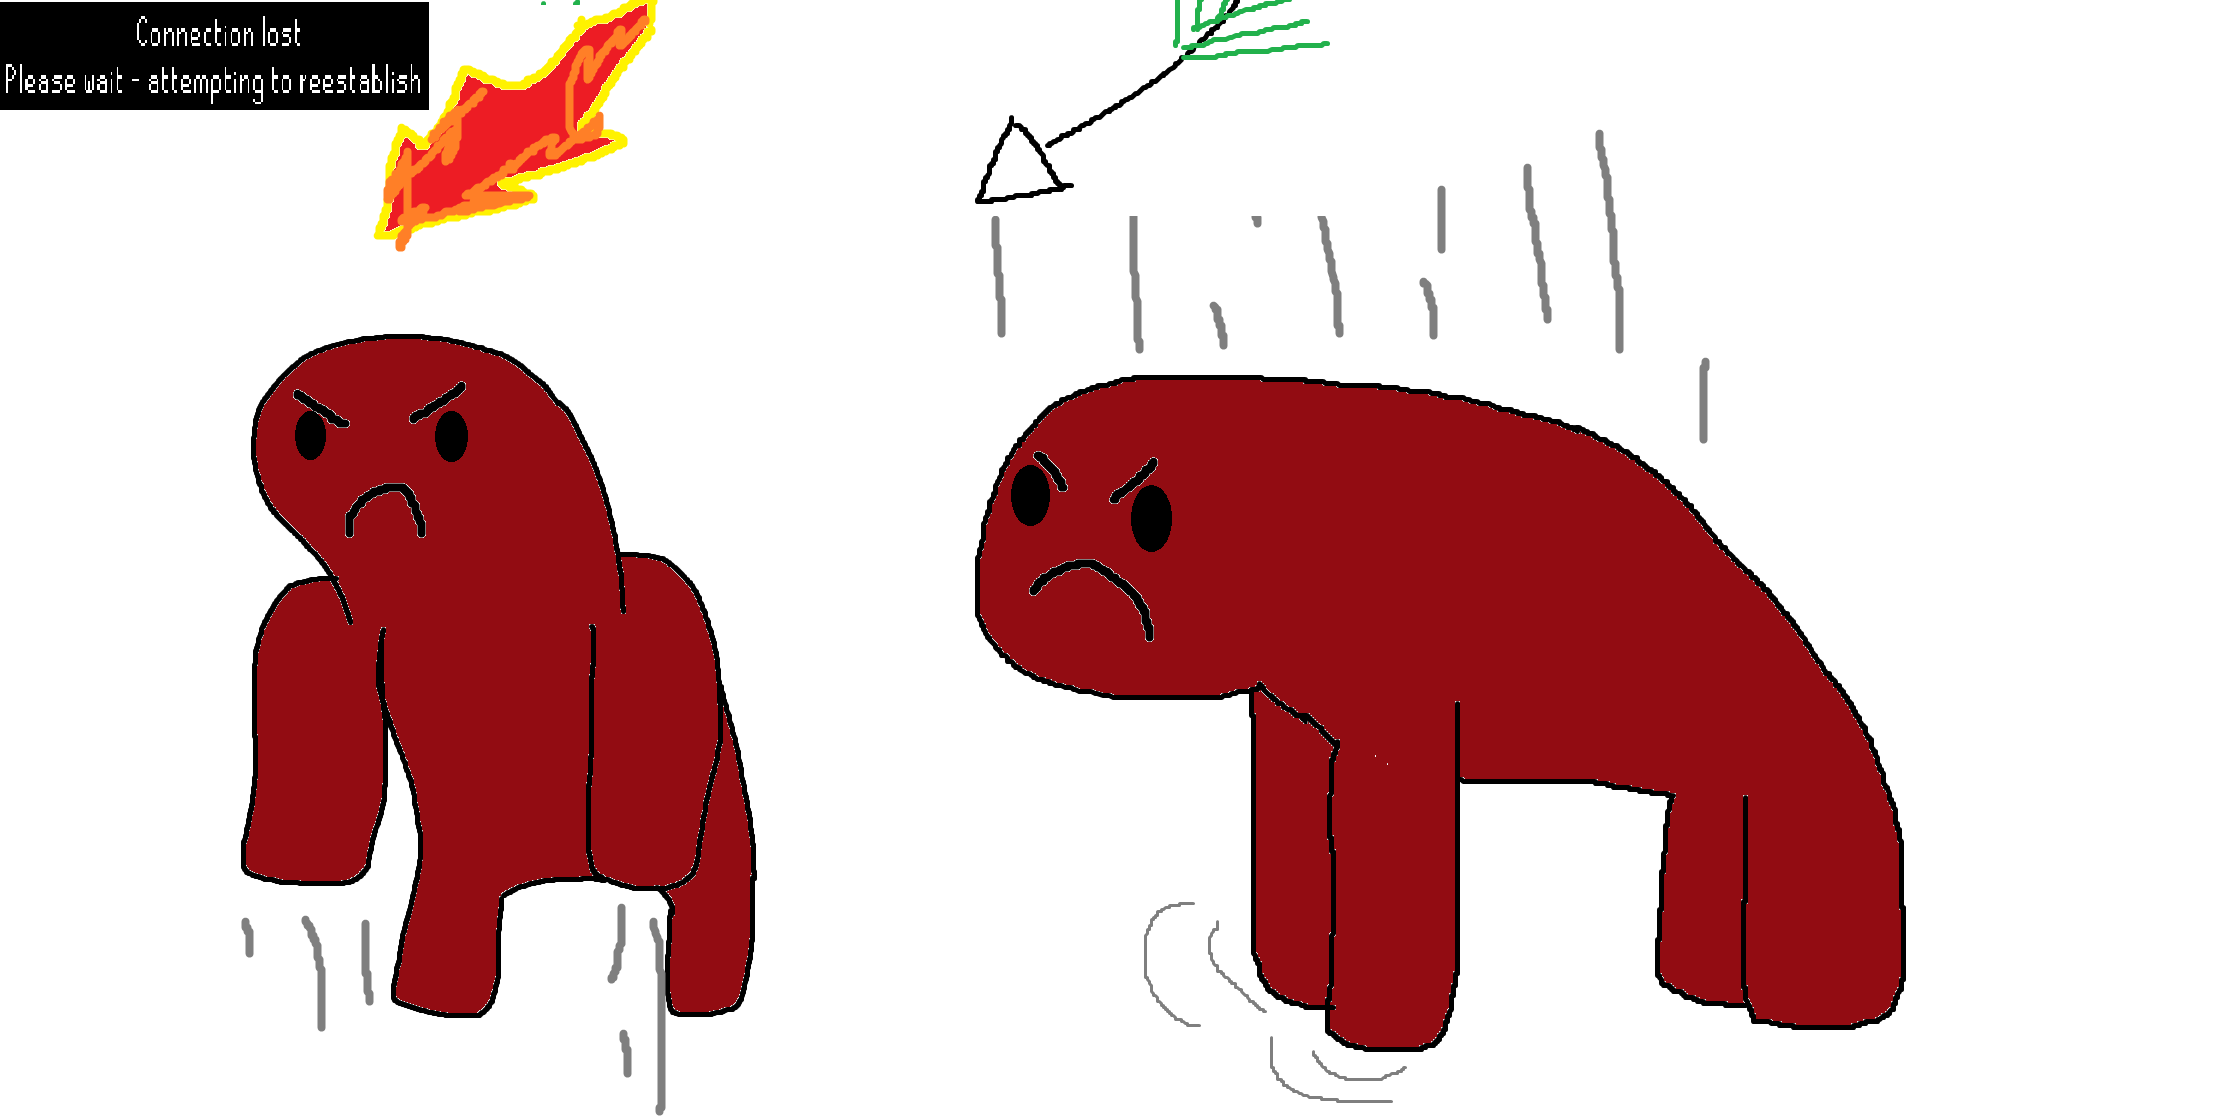
\includegraphics[scale = .3]{jadfight.png}
\end{figure}
\newpage
\subsection{Half HP \& Healers}
\begin{wrapfigure}{R}{.1\textwidth}

\includegraphics[width=.2\textwidth]{yt2.png}
\small \caption*{Healers}
\end{wrapfigure}
When you get Jad to half HP, 4 of his healers will come out. The goal to keep them from healing Jad back to full HP is to aggro them and have the healers focus on attacking you instead of healing Jad. However doing so will make it a little more straining on managing on prayer flicking and as well as your HP and prayer. Just make sure your HP isn't too low. The key  way to go about this is to auto one of the healers once, prayer flick for Jad, then re-position yourself to auto another healer. This cycle continues until you have all the aggro from the 4 healers. Make sure to move away from Jad a little so the healers aren't close enough to heal him. You also have the choice to kill the healers of you're having too much trouble dealing with them but it is more time consuming and the healers will respawn back. Get used to the cycle of drinking your brews, super restores, and prayer flicking and don't break it! The Fire Cape is just within your grasp now!
\subsection{Tips \& Tricks}

If you're having trouble fighting Jad, here are some tips you can try yourself.
\begin{itemize}
    \item If you're having trouble prayer flicking in time for Jad, there is a Jad simulator you can practice in. Link: \href{https://runeapps.org/jadsim_app}{Jad Sim}
    \item Too avoid from taking too much damage from the healers, you can reposition yourself between every Jad attack to align the healers in a line. Now only 1 healer will be dealing aggro since all the other's are blocked from hitting you! \textbf{Only do this if you're confident in prayer flicking!}
    \item Before fighting, make sure to have your combat style selected on \textbf{Long-Ranged}, This is to ensure that you won't get close enough to Jad so that he'll bite you! For extra measures if you have the brews/restores to do so, you can also keep on the prayer \textbf{Eagle Eye} to extend your range. 
    \item To keep yourself from accidentally moving towards Jad or displacing yourself by left clicking, be sure to always right click on your targets to attack them! This goes especially with the healers when they start coming out.
    \item If you find yourself too nervous and shaky before the fight, hide behind the rocks opposite to where the orange 360 mager spawned and give some time to collect yourself. Pot up, even out your breathing and remember to pray range when approaching Jad for the first time!
    \end{itemize}
\newpage

\section{Horray!...Now What?}
\begin{wrapfigure}{L}{.3\textwidth}
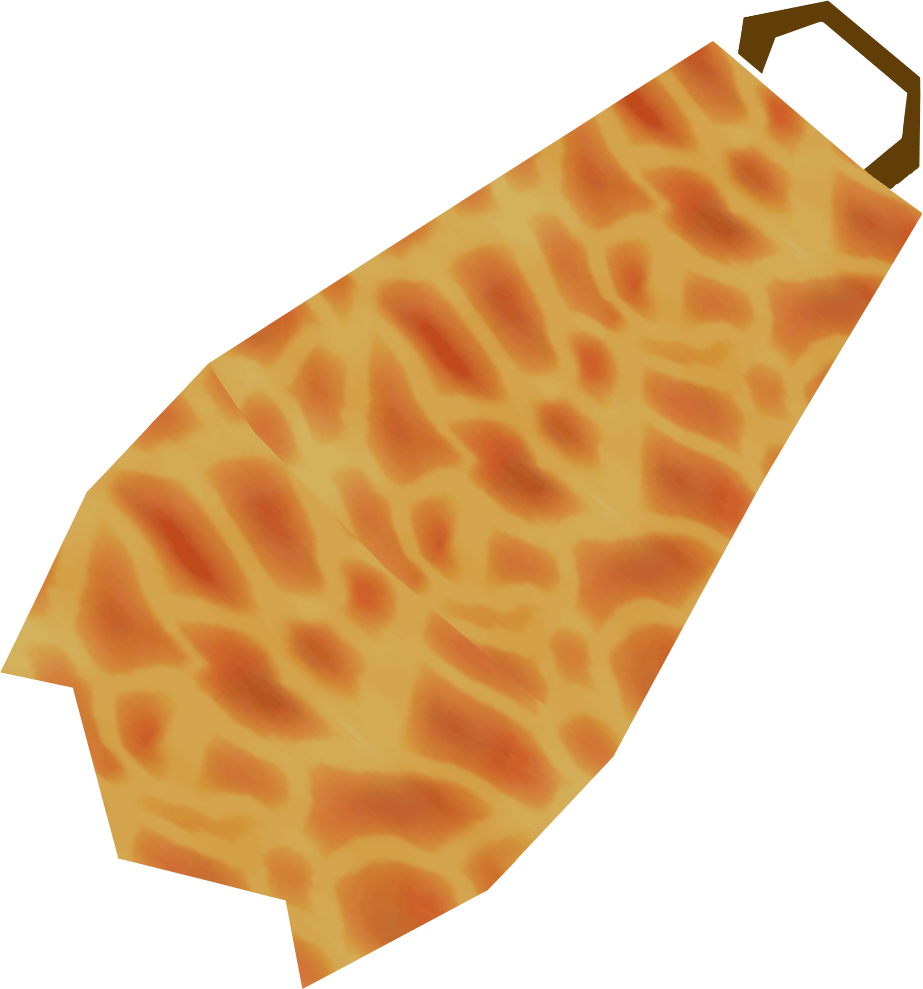
\includegraphics[width=.2\textwidth]{firecape.png}
\end{wrapfigure}
If you're reading this far, congratulations! You've been awarded the Fire Cape and are probably walking all around the game showing it off! After this long tolling and tedious journey, you're probably asking yourself, "Now what?"
\begin{figure}[!h]
    \centering
\centering

\includegraphics[width=.2\textwidth]{wahoo.png}\hfill

\includegraphics[width=.2\textwidth]{nice.png}\hfill

\includegraphics[width=.2\textwidth]{yay.png}
\end{figure}
\\Well, that is the beauty of this game--you can do anything after this! Maybe you just want to AFK and chill farming up a skill, or do fun quests with friends to blow some steam off, the choices are endless! Now, go on embark on your own adventures!
\begin{figure}[!h]
    \centering
    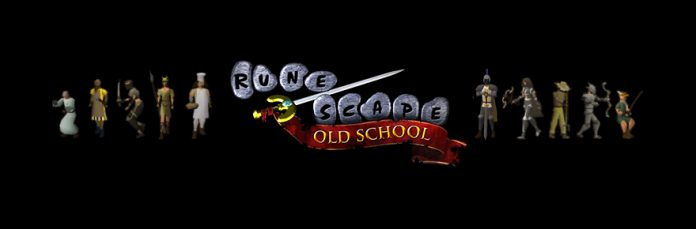
\includegraphics[scale = .7]{banner.jpg}
\end{figure}
\end{document}